\documentclass[sigplan,screen]{acmart}
\usepackage{listings}
\usepackage[ruled,vlined,lined]{algorithm2e}

%%
%% \BibTeX command to typeset BibTeX logo in the docs
\AtBeginDocument{%
  \providecommand\BibTeX{{%
    \normalfont B\kern-0.5em{\scshape i\kern-0.25em b}\kern-0.8em\TeX}}}

\begin{document}

\title{Generating Question Templates from a Knowledge Graph to Improve Coverage}

\author{Alex Gagnon}
\email{alex.gagnon@carleton.ca}
\affiliation{%
  \institution{Carleton University}
  \streetaddress{1125 Colonel By Drive}
  \city{Ottawa}
  \state{Ontario}
  \postcode{K1S-5B6}
}

\renewcommand{\shortauthors}{Gagnon}

\begin{CCSXML}
  <ccs2012>
     <concept>
         <concept_id>10002951.10002952.10003219</concept_id>
         <concept_desc>Information systems~Information integration</concept_desc>
         <concept_significance>300</concept_significance>
         </concept>
     <concept>
         <concept_id>10002951.10003227.10003351</concept_id>
         <concept_desc>Information systems~Data mining</concept_desc>
         <concept_significance>300</concept_significance>
         </concept>
     <concept>
         <concept_id>10002951.10003260.10003309</concept_id>
         <concept_desc>Information systems~Web data description languages</concept_desc>
         <concept_significance>500</concept_significance>
         </concept>
     <concept>
         <concept_id>10002951.10003317</concept_id>
         <concept_desc>Information systems~Information retrieval</concept_desc>
         <concept_significance>500</concept_significance>
         </concept>
     <concept>
         <concept_id>10010147.10010178.10010179</concept_id>
         <concept_desc>Computing methodologies~Natural language processing</concept_desc>
         <concept_significance>500</concept_significance>
         </concept>
   </ccs2012>
\end{CCSXML}

\ccsdesc[300]{Information systems~Information integration}
\ccsdesc[300]{Information systems~Data mining}
\ccsdesc[500]{Information systems~Web data description languages}
\ccsdesc[500]{Information systems~Information retrieval}
\ccsdesc[500]{Computing methodologies~Natural language processing}

\keywords{datasets, information retrieval, data description languages}

\maketitle

\section*{Abstract}

Given any store of information, a person or process must be able to query the store to extract data in a meaningful way for it to be usable. Compared to computer processes, however, humans are much looser with the mechanism in which they perform a query. A person structures their query as a question in some human language, whether in text or verbally. Converting this natural language question into something that can be executed against the data store and return the desired response is known as Question-Answering. Two common ways of completing this task are semantic parsing and templating. Semantic parsing decomposes the sentence into its grammatical substructures, allowing the parser to identify tokens such as nouns and verbs and use them to create a structured query to the store. Templating involves pre-generating pairs of natural language sentences and its structured query representation that can be executed against the datastore. The question is compared to the set of templates, and the most similar one is executed. Semantic parsing suffers from having a large learning period and is prone to bias while templating can have limited coverage as it is done using a specific text corpus. We seek to address the coverage issue by generating high-quality simple question templates that a generated directly from the knowledge base. We present two contributions: a mechanism to produce a large number of question templates, and RDFQA, a Python-based CLI application with a focus on user experience that performs Question-Answering tasks. The source code is made freely available\footnotemark

\footnotetext{\url{https://github.com/alexgagnon/big-data-final-project}}

\section{Introduction}

The domain of Question-Answering boils down to an inconsistency between the unstructured natural language-based question and the structured schema of the knowledge base that contains the answer. For example, given the question "where was Michael Jordan born?", a system is expected to be able to return the answer "Brooklyn, New York" in a timely manner. The concept of question and answering itself is vital for two reasons. First, a store containing potentially the entirety of collected human knowledge is, by itself, useless. A mechanism to extract facts in a generic manner, such as through voice or written text, is essential to give meaning to the data. Secondly, as more information is collected over time, the search space containing the possible answers becomes enormous. A strategy for question answering that performs quickly and accurately at scale, ideally in near-real-time, is the desired outcome for most applications.

When a question is asked in human language, a processing step must convert its semantics into a formal query suitable to be run against a datastore such as DBpedia, Freebase, or Wikidata. The information in these stores is represented by a graph containing facts in the form of subject/predicate/object triples, known as RDF (Resource Description Framework). For example, (Michael Jordan, birthPlace, Brooklyn NY), is an RDF triple, where "Michael Jordan" is the subject, "birthPlace" is the predicate, and "Brooklyn, New York" is the object. The primary mechanism for accessing these knowledge graphs is through specialized query languages (e.g. SPARQL), that traverse the graph and retrieve triples matching the request.

A failure to convert the question into the appropriate formal query will lead to incorrect answers. The likelihood of an erroneous conversion increases as the question becomes more complex. This can occur in several situations. Firstly, when a question is composed of multiple clauses (i.e. a conjunctive 'and', or through nested questions where the answer of one clause is used sequentially as input in the next). Secondly, the intricacies of the language itself can cause ambiguities, such as when pronoun usage makes the subject difficult or impossible to identify (e.g. 'John has a son named Tom, and he went to Harvard'.)

There are two standard approaches to solving this conversion problem: semantic parsing and templates.

\textbf{Semantic Parsing}. Semantic parsing deconstructs the question into one or more subgraphs based on the grammatical and syntactical structure of the sentence and then attempts to find matches in the knowledge graph. This strategy can be effective as it is, in essence, 'real-time' and does not require a large bank of previously computed examples. However, it is prone to incorrect subgraph creation. This is due to the fact that neural networks are typically used, which require a large and diverse set of training data to account for all topologies of subgraphs that exist in the knowledge base.

\textbf{Templates}. Template-based approaches instead try to convert the question into one or more simpler questions, which can be compared for similarity to a set of previously generated templates. Each of the question templates has an associated query which when executed against the knowledge graph will return the answer to the question. For example, a question such as 'what is the name of the person who has won the most NBA MVP awards ever' can be simplified to 'who has won the most NBA MVP awards'. This simpler question can be compared against a set of templates, and if a match is found, the associated query can be executed to find the answer. Templates have been found to be effective in returning high-quality answers in a timely fashion, however, they often suffer in coverage. Zheng et al. were able to outperform state-of-the-art implementations using binary templates. However, the source of the natural language templates was gathered through examining a single text corpus. As such, it suffered a lack of generalizability to other sources. It also uses neural networks to create simplified questions, which as previously mentioned depends on having accurate and diverse training data. This requirement can be limiting given that only a sole source in a specific domain is used.

We seek to address the issues of limited coverage for template-based approaches by instead generating natural language/query pattern pairs starting from the knowledge base itself. By traversing the triple graph, we can effectively create simple questions that map to any existing triple. For example, given the triple (Michael Jordan, birthPlace, Brooklyn), we can create simple questions to represent it such as 'where was Michael Jordan born' or 'which city was Michael Jordan born in', and its corresponding SPARQL queries 'Michael Jordan, birthPlace, <?>'. More general questions stemming from the subjects and objects can also be produced, such as 'who is Michael Jordan', and 'where is Brooklyn', which further complete the search space. Of course, such precision in templates covering the entire knowledge graph entails having an enormous amount of templates, causing a huge memory footprint and search time. The use of question words (e.g. when, where, who, what, why, how) can be injected based on the types of entities and classification of predicates found in the triple. Similar 'bottom-up' approaches of starting from the knowledge base itself include work by \citeauthor{generating-factoids}, where a large corpus of question-answer pairs was created. The goal in this case, however, was to produce question-answer pairs for use in benchmarking and not for use as templates.

In order to confirm whether or not the repository of templates we produce are accurate question-query pairs, we also created RDFQA, a CLI-based Question-Answering application. The application is focused on being user-friendly, allowing a user to enter a natural language question. It also provides tuning parameters to allow for easily configuring the operation of the application.

\textbf{Contributions}

\begin{itemize}
    \item a collection of template pairs, consisting of a question template and the structured SPARQL query that it represents
    \item RDFQA, a user-focused Question-Answer application that uses the generated template pairs
\end{itemize}

\section{Background}

Question-Answering involves numerous domains of computer science. First, natural language processing (NLP), is required to semantically analyse a question. Second, an ontology is used to provide a structured means of labelling concepts and relationships among entities. For example, Resource Description Framework (RDF) and OWL provide the necessary specifications to create a semantic web, where data can be refined to a given class of concept, a certain data type, allowable range values, etc. Third, the data records must be stored in a database that is conducive to handling enormous amounts of data by storing them as graphs (known as Knowledge Graphs or Knowledge Bases). Fourth, specialized query languages are used to interact with the knowledge graphs, notably SPARQL, an SQL-like language that is terse yet expressive enough to query the vast amounts of data in a store. We will provide additional details of these subjects in the following sections.

\subsection{Natural Language Processing}

Natural Language Processing is the field of Artificial Intelligence that allows computers to operate on human languages. It is not trivial to dissect some corpus or sentence into its constituent parts, but it is a necessary step for understanding it's meaning. There are numerous goals in NLP depending on which parts of the text are of interest:
\begin{itemize}
    \item \textbf{Tokenization} - identifying pieces of text, like entities (nouns), verbs, adjectives, etc., also known as Parts Of Speech.
    \item \textbf{Stemming} - finding the 'stem' of a word, useful to identify variations of a word (i.e. 'comput' is the stem of compute, computed, computer, computing, etc.). The stem need not be a real word.
    \item \textbf{Lemmatization} - similar to 'stemming', but the root is actually a word (i.e. 'compute' is the lemma of computer, computed, computing, etc.)
\end{itemize}

For example, running the sentence 'where was Michael Jordan born' through an NLP tokenizer might identify that 'Michael Jordan' is a noun (an entity representing a thing), 'born' is a verb, 'where' is a preposition, etc. See Table \ref{table:tokenization} for example output from spaCy, a common Python NLP library.

\begin{table}[]
\caption{Sample output of the phrase 'where was Michael Jordan born' being entered into spaCy's \texttt{nlp} function}
\label{table:tokenization}
\begin{tabular}{|l|l|l|l|l|}
\hline
Text    & Lemma   & Part Of Speech & Tag  & Stop Word \\ \hline
where   & where   & adverb         & WRB  & true      \\ \hline
was     & be      & auxiliary      & VBD  & true      \\ \hline
Michael & Michael & proper noun    & NNP  & false     \\ \hline
Jordan  & Jordan  & proper noun    & NNP  & false     \\ \hline
born    & bear    & verb           & VERB & false     \\ \hline
\end{tabular}
\end{table}

\subsection{Ontologies}

With so much content available on the Internet, it becomes crucially important to have a well-defined and agreed-upon standard for representing information. An ontology, a.k.a a 'vocabulary', gives the ability to provide additional semantic information about an entity and it's relationships to other entities. In the case of structured linked data, the \href{https://www.w3.org/standards/semanticweb/ontology}{W3C provides several ontologies} geared towards different uses cases. RDF and OWL are the most common frameworks for linking data together and giving it semantic meaning. Both the RDF and OWL specifications group together a subject, a property (also known as a predicate), and an object into a single tuple known as a 'statement' or 'triple'. OWL is a more expressive framework than RDF as RDF provides a smaller, looser vocabulary, while OWL gives a larger vocabulary to define things, finer-grained constraints on the data, and is more strict. For example, in OWL you are able to restrict data elements to a given data type (e.g. integer, float, string, boolean, etc.), which provides much more expressivity. A property may have restrictions on the subjects and objects it can relate, providing not only more accurate meta-information but the means for more expressive querying.

Elaborating on the previous example, (Michael Jordan, birthplace, Brooklyn), is one such statement for both RDF and OWL. This statement by itself is useful, however, the true power of semantically linked data is that each of these elements can be referenced by other statements, forming a web of interconnected entities. For example, other statements linked together by these elements would be (Michael Jordan, played for, Chicago Bulls), and (J. K. Rowling, birthplace, Gloucestershire).

Similarly to traditional RDBMS systems, having a unique identifier for each record in a store instead of a text label is important for it to be consistently referenced. Both RDF and OWL use URIs, typically in the form of URLs, as identifiers. The example above using URIs in the DBpedia knowledge graph would be:

\begin{lstlisting}[breaklines=true]
(
  <http://dbpedia.org/resource/Michael\_Jordan>,
  <http://dbpedia.org/ontology/birthPlace>,
  <http://dbpedia.org/resource/Brooklyn>
)
\end{lstlisting}

While these URIs are essential as unique qualifiers, they are geared towards computers. Humans use natural language to refer to things, often with many variations and ambiguities. For example, 'birthPlace' can be represented in English as the direct label 'birthplace', but also by 'place of birth', 'born in', 'place they were born', etc. Being able to determine a URI based on every possible variation of their label has proven to be difficult, and many authors attempt to solve this through machine learning applications such as neural networks \cite{zheng-question-over-knowledge-graph,zheng-how-to-build-rdf-templates,complex-questions-over-knowledge-bases}.

One important consideration for properties when dealing with querying is that there are two common forms:

\begin{itemize}
    \item \textbf{has} - this form of property says the subject 'has' the given object as a kind of property
    \item \textbf{is instance of} - the subject is a kind of property of the object
\end{itemize}

This can lead to confusion, as we will see in the Implementation and Results section.

\subsection{Knowledge Graphs}

Knowledge bases are the computational representation of a group data related to a certain domain. They store either structured or unstructured data in a persistent store, Contrary to traditional relational databases, they are concerned with representing facts about the domain, which require different storage techniques than normalized tables approach of RDBMSes. The Internet itself is an example of one giant knowledge base, as it is composed of billions of documents hyperlinked together. Other projects have emerged which attempt to store factual information in a knowledge base, such as:

\begin{itemize}
    \item \textbf{Wikidata} - a free and open database that, while useful in isolation as a knowledge graph, supports additional Wikimedia projects such as Wikipedia
    \item \textbf{DBpedia} - a knowledge store built by querying the structured data stored in Wikipedia article infoboxes.
    \item \textbf{Freebase} - Freebase was one of the leading knowledge bases before being purchased by Google. The technology behind it is now used to power the infoboxes for Google's search engine.
\end{itemize}

In these knowledge bases, the facts are stored as RDF triple statements and can be represented as a graph. Each of them allows for operations like creating new nodes and performing queries to find relationships between the nodes. Figure \ref{fig:knowledge_graph} demonstrated our running example of (Michael Jordan, birthPlace, Brooklyn), as well as how relationships between entities can be identified (both Michael Jordan and Scotty Pippin played for the Chicago Bulls.)

\begin{figure}[h]
    \includegraphics[width=\columnwidth]{knowledge-graph.png}
    \caption{An example knowledge graph}
    \label{fig:knowledge_graph}
\end{figure}


\subsection{SPARQL}

SPARQL is the W3C recommended querying language for RDF-based ontologies, however, it can also be used with other ontologies such as OWL. It is SQL-like, in that it contains familiar syntax like 'select' for projections and 'where' for conditional clauses. However, it differs in that the conditional clauses define triple patterns representing the various elements of a triple. One or more of the elements can be replaced with variables, allowing the SPARQL engine to search through the database and return all statements that match the pattern. The arguments are positional, such that the pattern \texttt{\{?s ?p ?o\}} represents the subject, property, and object, respectively (in this case, all the elements are free variables and as such every triple in the database is a match). For example, figure \ref{figure:sample-query} represents a SPARQL query to DBpedia that returns the birthplace of Michael Jordan in JSON format.

\begin{figure}[h]
\begin{lstlisting}[language=SPARQL,frame=single,breaklines=true]
select ?o where {
  <http://dbpedia.org/resource/Michael_Jordan>
  <http://dbpedia.org/ontology/birthPlace>
  ?o
}
\end{lstlisting}

\begin{lstlisting}[frame=single,breaklines=true]
{
  "head": {
    "link": [],
    "vars": [
      "o"
    ]
  },
  "results": {
    "distinct": false,
    "ordered": true,
    "bindings": [
      {
        "o": {
          "type": "uri",
          "value": "http://dbpedia.org/resource/Brooklyn"
        }
      }
    ]
  }
}
\end{lstlisting}
\caption{Sample SPARQL query to find where Michael Jordan was born, and the response as a URI, in JSON format}
\label{figure:sample-query}
\end{figure}

\section{Implementation}

The contributions in this paper are two-fold: a method of generating question/SPARQL query pairs, and a CLI application which uses the template pairs to perform QA tasks. The template generation phase occurs completely offline, while the application provides a real-time interface. The implementation details for the two solutions are as follows.

\subsection{Offline Automatic Template Generation}

The central idea governing the template-generation strategy is to provide some set of templates that a question can be compared to for similarity. During template generation, a question template and a SPARQL query are created, where the query contains the necessary triple patterns and filters to answer the question. As in all computer science problems, a determining factor in the effectiveness of the system is the use of space and how quickly it runs. The more templates that are available, the more likely it is to find a very similar match, which should produce a more accurate resulting answer. However, more templates also mean a larger memory footprint, and more elements to search through. Both are highly dependant on the data structures and algorithms used to store and search the templates.

Unlike \citeauthor{zheng-question-over-knowledge-graph}, who generate templates based on a single corpus document, we use the knowledge base itself as the source of information. Conceptually, since each triple in the graph contains a URI for a subject, a property of that subject, and the corresponding object, by replacing one or more of these in a question we can generate representative templates. For example, consider the question: where was Michael Jordan born? This is composed of a question word 'where', an auxiliary verb 'was', and entity 'Michael Jordan', and a property 'born' (which as discussed in section 2.3, is a label corresponding to the property 'birthPlace'). We seek to create a minimal template of this question, which can be interpolated with the corresponding URIs at runtime. A template question and corresponding SPARQL query which would be considered highly similar to this question is given in Figure

\begin{figure}
\begin{verbatim}
    where was {subject} born,
    select ?o where {
      <subject\_URI>
      <http://dbpedia.org/ontology/birthPlace>
      ?o
    }
\end{verbatim}
\caption{Example question-query template pair, trying to identify where a given subject is born (the subject's URI is interpolated at runtime)}
\label{figure:question-query-pair}
\end{figure}

Theoretically, we could scour the entire knowledge base and retrieve the labels (and their variations) for all possible entities and properties. This would allow generating a complete set of question templates that cover all the statements in the knowledge base. In this scenario, for simple questions, the question template itself would have no variables, and the SPARQL query would have a triple pattern where the URIs are already hard-coded (see Figure \ref{figure:sample-query} for how this would look with the (Michael Jordan, birthPlace, ?) example). However, in this case, the number of templates would be prohibitively large, making this an unlikely strategy unless highly efficient indexing and filtering strategies were used.

Our implementation instead tries to take a balanced approach by creating partially complete templates based on the available properties in the knowledge graph. We pre-generate a set of templates where the subject's URI is not fixed, but the question contains actual property labels. Figure \ref{figure:question-query-pair} is an example of this approach, since 'born' is a reference to 'birthPlace', but '{subject}' is determined and replaced at runtime by RDFQA, discussed in section 3.2.

The templates are created by having a set of manually curated questions which may contain placeholders for where the properties would be found (in the current implementation, represented by '{property}'. Some example question prototypes could be 'what is {subject}', 'when did {subject} {property}', etc. We query the database to retrieve both the URI and the label of all of the available properties. To reduce the number of invalid question templates, we place some additional constraints on the query. First, we use OWL, as it's richer vocabulary allows us to classify the properties by their data type. For example, the subject of any statement with the 'birthPlace' property should be restricted to living things such as a Person, while the object should be a Place (Person and Place are capitalized since they represent classes in OWL and RDF). Second, we perform a secondary query to the database to count the number of times a property is actually being used. Since we are trying to reduce the number of templates we produce, we want to be able to restrict our templates to those that have high value. The RDFQA application provides a mechanism to control this parameter by setting a required minimum number of references and discards any properties that do not meet the threshold.

The final step is to iterate over our manual question prototypes and the properties to create the question-query pairs. The '{property}' placeholder from the question prototype is replaced with the properties' label, and the SPARQL query is generated where the property variable is replaced with its URI (exactly as can be seen in Figure \ref{figure:question-query-pair}). Since the properties were restricted by data type, we are able to use these types to reduce the number of nonsensical question templates. By classifying the question prototypes as having specific types of answers (i.e. where was {subject} born -> Place), we are able to restrict the prototypes to only those properties whose data types are consistent with the desired range. The resulting pairs are outputted to a JSON file for subsequent use.

We discovered that certain question prototypes do not require a '{property}' placeholder at all, as the property can be directly inferred by the form of the question. For instance, the question 'who is Michael Jordan' suggests the answer should be a summary or description of Michael Jordan. As such, these question prototypes were not iterated over, but have a one to one mapping with a question/query template.

The steps involved in the template can be seen in Algorithm \ref{figure:template-generation}

\begin{algorithm}[h]
\SetAlgoLined
\KwData{
 $Q \longleftarrow$ set of prototype questions\;
 $R \longleftarrow$ set of queries for property-less prototype question\;
 $P \longleftarrow$ set of properties in cache\;
 $D \longleftarrow$ set of OWL data types used to constrain the properties\;
 $\sigma \longleftarrow$ minimum number of references required for a property\;
}
\KwResult{$T$ :a set of template-question/SPARQL-query pairs}
\Begin{
 \state{$T \longleftarrow []$}\;
 \If{$P = None$}{
   \state{$P \longleftarrow$ get\_all\_properties()}\;
 }
 \state{$F \longleftarrow$ filter\_properties($P, \sigma$)}\;
 \For{$q \in Q$}{
     \If{$q$ has no property placeholder}{
       \state{T.append($R$[$Q$])}\;
     }
     \Else {
     \For{$f \in F$}{
       \For{$d \in D$}{
          \state{T.append(generate\_template\_pair($q, f$)}\;
        }
     }
 }
 }
 \state{return T}\;
 }
 \caption{Template question generation}
 \label{algo:template-generation}
\end{algorithm}

\subsection{Online Question Decomposition}

While having a collection of templates is good, we also seek to be able to use them to perform QA tasks. As such, we also contribute RDFQA, a Python-based CLI application that uses the templates produced by the template-generation phase to answer questions in real-time. A focus on the application was to make it user-centric, allowing the runtime parameters to be easily modifiable through either a configuration file or via command-line arguments.

The process is as follows. First, the user inputs a question either as a command-line argument or through the REPL interface provided by the application. The question is parsed by an industry-leading natural language library (spaCy), which decomposes it into its grammatical parts. Of note, we seek to identify the entities in the question (i.e. the proper nouns), of which one is the subject. Figure \ref{figure:sentence-deps} and \ref{figure:sentence-ents} demonstrate the results of the grammatical dependencies and named entity recognition used to identify relevant parts of the question. We use a SPARQL HTTP endpoint to lookup the corresponding URI for the subject. The question is parsed, replacing the subject with the corresponding placeholder used in the templates. If in the question prototypes the string '{subject}' is used, then the question is converted to replace the subject with the equivalent placeholders. For example, in the question 'where was Michael Jordan born', Michael Jordan would be identified as the subject, the question would be converted to 'where was {subject} born' since '{subject}' is the placeholder used in the question templates. The URI of Michael Jordan would be found in order to replace it in the matching templates' SPARQL query.

Next, the set of templates is iterated over to try and find similar templates. Configuration options are available, so as to return only those templates with a similarity above a certain threshold, to return the top-k similar results, and which algorithm to use to compare similarities. Currently, the two algorithms are the one provided by spaCy, and Levenshtein edit distance. These differ in their approach, as the NLP library attempts to match based on grammar and semantic meaning, while the edit distance is strictly about character differences.

If one or more similar templates are returned, the SPARQL queries are then executed. The subject URI in the SPARQL query is replaced with the URIs found in the question decomposition step above. Since an entity may be referenced by more than one URI, several different combinations are iterated over, up to a configurable maximum number of attempts.

If an answer is found, it is returned to the user.

The pseudocode for the operations is given in Algorithm \ref{algo:rdfqa}.

\begin{figure}[h]
  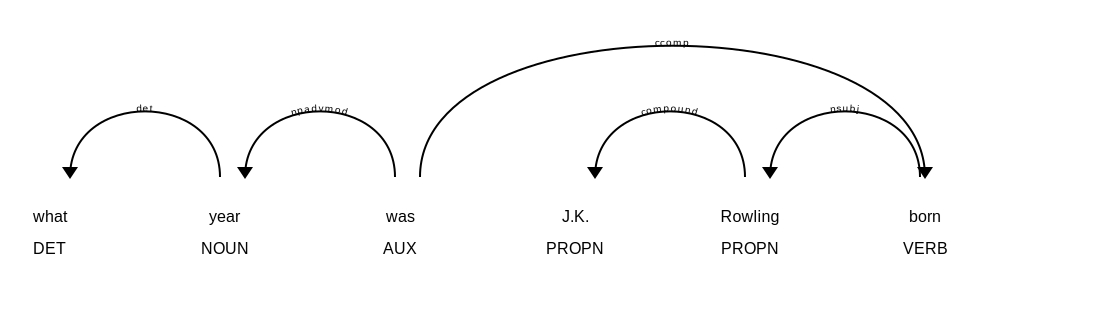
\includegraphics[width=\columnwidth]{sentence-deps.png}
  \caption{Grammatical deconstruction of the question 'where was Michael Jordan born' via the spaCy library}
  \label{figure:sentence-deps}
\end{figure}

\begin{figure}[h]
  \includegraphics[width=\columnwidth]{sentence-ents.png}
  \caption{Named entity recognition of the question 'where was Michael Jordan born' via the spaCy library}
  \label{figure:sentence-ents}
\end{figure}

\begin{algorithm}[h]
\SetAlgoLined
\KwData{
 $Q \longleftarrow$ question being asked\;
 $T \longleftarrow$ collection of pre-generated templates\;
 $\theta \longleftarrow$ maximum number of iterations\;
}
\KwResult{$a$: the set of potential answers}
\Begin{
 \If{$T = None$}{
   \state{$T \longleftarrow$ generate\_templates()}\;
 }
 \state{$q, e \longleftarrow$ convert\_question\_to\_template(Q)}\;
 \state{$t \longleftarrow$ get\_similar\_templates(q)}\;
 \state{$e \longleftarrow$ get\_entity\_URIs(e)}\;
 \state{$a \longleftarrow$ None}\;
 \For{$i \longleftarrow$ 0 to $\theta$}{
  \state{$a \longleftarrow$ get\_answer($q, t[i]$)}\;
  \If{$a \neq$ None}{
    \state{return $a$}\;
  }
 }
 \state{return None}\;
 }
 \caption{RDFQA question-answering}
 \label{algo:rdfqa}
\end{algorithm}

\section{Experimentation}

In order to test the effectiveness of RDFQA, benchmarks are included in the application. The benchmark questions are taken from a fork of a set of simple questions for Wikidata. However, an issue became apparent in the sample datasets. First, all capitalization has been removed. Capitalization is crucial to being able to detect proper nouns in a sentence, and therefore the NLP library used to decompose the question failed to detect any subject. Therefore, we modified the benchmark to 50 hand-curated questions, where the proper nouns have been capitalized.

\section{Results}

Unfortunately, the results of RDFQA are unimpressive. Despite simplifying the benchmarks to help the NLP library, the application failed to provide the correct answer in the vast majority of cases. Additionally, the lack of an efficient lookup algorithm means that the queries are quite slow given any meaningful number of templates. Visual inspection of the output of the benchmarks provides some insights, however.

First, there remains an issue where the NLP library is unable to identify the subject in certain situations. Notably, two such occurrences become evident. First, when the proper noun contains initials, for example, J.K. Rowling. In this case, the library may terminate at one of the periods, as opposed to treating the name as a complete entity. Secondly, when the possessive 's is used, often it is included in the name, cause the URI lookup to fail. For example, varying our running example to 'what is Michael Jordan's place of birth', the library detects Michael Jordan's as the entity. Of course, Michael Jordan is the correct entity here. When additional filtering was attempted in the query to try and accommodate this (i.e. using SPARQL's native filtering functions of regex or contains), the query would often timeout. To combat this, a user is able to set a configuration parameter to remove all possessive 's instance in the questions. Anecdotally, this appears to fix the majority of cases when a question is asked ad-hoc, however, it did not drastically improve the results of the benchmarking.

Secondly, the variations of the labels for the properties often were not sufficient to result in strong similarity. For example, the two sentences 'where was Michael Jordan born' and 'what is Michael Jorda's place of birth' are identical semantically: they both seek the location of MJ's birthplace. While the edit distance similarity metric would be of no use, in this case, the NLP libraries' similarity function would be expected to identify this as extremely similar. Results indicate that this was not the case however, as often the same property in a different tense was not considered similar at all. Several solutions for this exist. Certain properties contain variations directly in the knowledge base, such as 'bornIn' redirected to 'birthPlace' During template generation, when we retrieve the properties from the knowledge base we could do some additional processing to retrieve all labels the redirect to the base form of the property. This would increase the number of templates, however, potentially slowing down the search speed. Another example would be to train the NLP's similarity model with a more specific set of training data, taken from the knowledge base. We did not investigate this option, however. Also related to errors with properties has to do with the aforementioned differences between 'is instance of' and 'has' variations. For properties that are of the 'has' form, the SPARQL prototype currently used correctly specifies the object as the desired result. For the 'is instance of' versions, such as <

Third, the issue with slow template searching. The NLP library used (spaCy) is geared towards industry use. As such, it hides its implementation details and only provides a simple API. The underlying mechanics such as which algorithm it uses are hidden from the consumer. Other libraries exist that are more suited to academic and research use, such as NLTK. In these packages, much more freedom is given to the developer as to the selection of algorithms. This has the potential to select similarity metrics that may perform better in the specific use case of template matching.

\section{Conclusion and Future Work}

Some improvements to the existing architecture could address some of its shortcomings. For example, to address the search speed for similar templates, novel algorithms have been introduced which provide faster speeds through contextual hashing. Locality sensitive hashing is one such algorithm where an object is hashed, but instead of a purely random outcome, it is bucketized based on the object's properties. We could use this to create context-sensitive hashes of the templates during the generation phase, which could provide linear time lookups for a question at runtime.

When looking up URIs for the question's subject, we struggled whenever the label differed slightly from those in the knowledge base (whether due to the possessive, initials, or otherwise). spaCy in fact already provides a means to include a knowledge base identifier out of the box, however, the additional features require upwards of 50GB of source files, and so were not tested in this release. This could be helpful since the more rigid filtering of subject labels using a regular expression often caused the query to timeout. Being able to determine if an entity has a URI through an in-memory store instead of through an HTTP request has the potential to both speed up searching and increase the accuracy of the application since timeouts would not exist.

For property errors, additional work on the algorithms could address the 'has' vs. 'is instance of' incompatibilities, wherein one the property is the subject and the other an object. As an alternative, the algorithm that retrieves all properties could be modified to include contextual and tense-based variations, at the expense of template search speed.

Template matching has the potential to greatly increase the accuracy and speed of question-answering tasks but often suffers from coverage and speed. We attempted to address these issues (especially coverage) by creating partial templates that cover the entirety of a given knowledge base. RDFQA was created to aid in providing a QA interface to use the generated templates. However, due to several difficulties, the current application is not competitive with state-of-the-art implementations.

\nocite{*}
\bibliographystyle{ACM-Reference-Format}
\bibliography{proposal-references}

\end{document}
\endinput
